Table~\ref{tab:pathtable} reports the primary comparison on the 96
test demand paths under the frozen protocol of
Section~\ref{sec:pairresults}: flow-prediction error, attribution-column
error, geometric-boundary error, and the number of paths improved by
response supervision. The unrestricted and integrated-bound columns
and their group-level breakdown move to
Table~\ref{tab:boundchain96} (Appendix~\ref{supp:learningdetail});
Appendix~\ref{app:pairs-v102} gives full objectives and denominators.
\begin{table}[t]\centering\footnotesize
\caption{Prediction and spatial explanation on the same 96 test demand
paths (24 per group). Entries are group medians of path-level values;
flow errors are additionally averaged over the 41 states within each
path. Geometric: the maximum account error over the geometric family,
as a percentage of the reference geometric-family maximum. Improved:
paths on which response supervision lowers the error.}\label{tab:pathtable}
\setlength{\tabcolsep}{4.5pt}
\begin{tabular*}{\tblwidth}{@{\extracolsep{\fill}}rcc cc cc cc}
\toprule
& \multicolumn{2}{c}{Flow pred.\ (\%)} & \multicolumn{2}{c}{Column (\%)} & \multicolumn{2}{c}{Geometric (\%)} & \multicolumn{2}{c}{Improved}\\
\cmidrule(lr){2-3}\cmidrule(lr){4-5}\cmidrule(lr){6-7}\cmidrule(lr){8-9}
Active & flow & resp. & flow & resp. & flow & resp. & col. & geo.\\
\midrule
1 & 0.032 & 0.029 & 8.13 & 4.92 & 2.95 & 1.78 & 24/24 & 23/24\\
2 & 0.032 & 0.029 & 21.09 & 15.67 & 8.62 & 6.19 & 22/24 & 21/24\\
3 & 0.033 & 0.029 & 21.53 & 15.46 & 9.07 & 6.01 & 22/24 & 22/24\\
6 & 0.033 & 0.030 & 22.45 & 14.22 & 9.27 & 5.77 & 24/24 & 24/24\\
\midrule
All 96 & 0.032 & 0.029 & 21.18 & 14.19 & 8.74 & 5.75 & 92/96 & 90/96\\
\bottomrule\end{tabular*}\end{table}
On the 96 test demand paths, response supervision lowers the median
attribution-column error from 21.18\% to 14.19\% (a relative reduction
of one third) and the geometric-boundary error from 8.74\% to 5.75\%,
while both models retain flow-prediction errors near $0.03\%$ (medians
$0.0322\%$ and $0.0292\%$). The improvement holds in every
active-query group. Path-level paired differences quantify the
uncertainty: the median paired column-error difference is $-5.03$
percentage points with a path-level bootstrap $95\%$ interval of
$[-6.01,-4.48]$ (10,000 resamples), improving 92 of 96 paths; the
paired geometric difference has median $-2.06$ with interval
$[-2.76,-1.65]$, improving 90 of 96, with every group's interval
excluding zero and leave-one-path-out medians varying within
$[-5.11,-4.94]$ and $[-2.11,-2.00]$
(Appendix~\ref{supp:learningdetail} reports the group-level intervals).
The system-contribution difference is secondary and opposite in sign
(median $+0.45$, interval $[0.01,0.74]$; both methods below $3.5\%$),
confirming that scalar completeness and spatial explanation accuracy
measure different properties. The same-path decomposition of
Eq.~\eqref{eq:coldecompmain} attributes the discrepancy to demand-response
error on every path--query pair (path--query median response and weight
norms $206.5$ and $3.5$ under flow supervision, $147.6$ and $3.3$ under
response supervision).

\paragraph{Six objectives under a fair weight search.}
Table~\ref{tab:fairmethods} completes the objective comparison under
the shared continuation budget and the common validation-only weight
search (Appendix~\ref{app:pairs-v102}). All six objectives train at a
properly selected weight. Weighted-response supervision --- the direct
form identified by the decomposition of
Eq.~\eqref{eq:coldecompmain} --- matches the unweighted objective it
approximates: their medians differ by less than half a percentage
point on every explanation metric (column error $13.85\%$ versus
$14.19\%$, with the lowest unrestricted boundary error among the
selected weights at $11.92\%$), confirming directly that the
weight-shift term the
unweighted objective ignores is small. The unweighted form remains the
practical choice: it attains the lowest flow error and geometric
error and tolerates the widest weight range, while beyond
$\lambda=0.03$ the weighted objective pushes the validation flow
error past the eligibility screen and selection falls back to the
initial checkpoint. The two endpoint objectives improve substantially
over flow-only training at their selected weight
($21.18\%\to16.2\%$ in column error), correcting the weak showing of
their earlier fixed-coefficient runs, but remain behind the response
family. The boundary-seminorm objective shows the largest
validation--test gap. Its validation boundary error decreases
monotonically with the weight up to the selected $\lambda^*=0.3$ and
reaches the lowest validation value of any objective, yet its test
column error at that weight stays above flow-only training
($24.18\%$, improved on only 8 of 96 paths); its smaller weights do
test better than flow-only training but are dominated on validation,
so the validation signal favours weights that do not transfer.
Optimizing the boundary value alone does not repair the underlying
response field, whereas supervising that field improves every spatial
error metric.
\begin{table}[t]\centering\footnotesize
\caption{Six supervision objectives on the same 96 test demand paths,
each at its validation-selected weight $\lambda^*$ under the shared
continuation budget and uniform selection rule
(Appendix~\ref{app:pairs-v102}). Entries are medians of path-level
values; improved: paths on which the objective lowers the column
(geometric) error relative to flow-only
training.}\label{tab:fairmethods}
\setlength{\tabcolsep}{5pt}
\begin{tabular*}{\tblwidth}{@{\extracolsep{\fill}}lcccc cc}
\toprule
Objective & $\lambda^*$ & Flow pred.\ (\%) & Column (\%) & Geometric (\%) & \multicolumn{2}{c}{Improved vs.\ flow}\\
\cmidrule(lr){6-7}
& & & & & col. & geo.\\
\midrule
Flow only & --- & 0.032 & 21.18 & 8.74 & --- & ---\\
Response supervision & 1 & 0.029 & 14.19 & 5.75 & 92/96 & 90/96\\
Weighted response & 0.003 & 0.032 & 13.85 & 6.17 & 91/96 & 90/96\\
Boundary seminorm & 0.3 & 0.037 & 24.18 & 7.21 & 8/96 & 45/96\\
Endpoint-edge & 0.3 & 0.035 & 16.23 & 7.46 & 72/96 & 66/96\\
Endpoint-cut & 0.3 & 0.035 & 16.26 & 7.47 & 72/96 & 67/96\\
\bottomrule\end{tabular*}\end{table}
\begin{figure}[t]
\centering
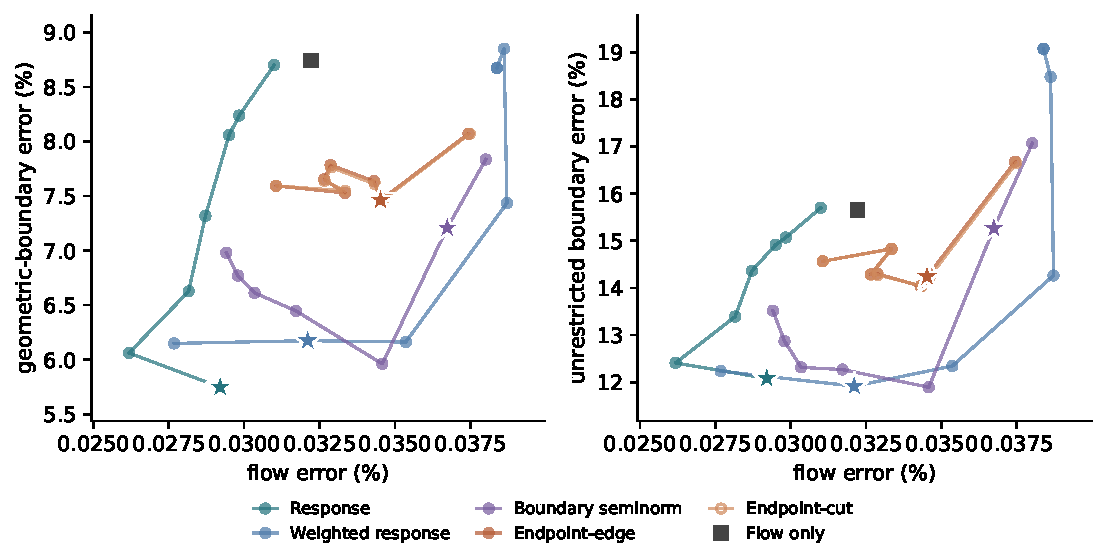
\includegraphics[width=\linewidth]{../figures/fig_v109_pareto.pdf}
\caption{Explanation--flow trade-off of the six supervision objectives
across the weight grid, on the 96 Sioux Falls test paths. Each point
is one (objective, weight) configuration: median flow error against
median geometric-boundary error (left) and unrestricted boundary error
(right); the validation-selected weight of each objective is starred.
Response supervision sweeps the efficient frontier in both panels,
interpolating between flow-only behaviour and the lowest geometric
error; weighted-response supervision matches it at small weights ---
attaining the lowest unrestricted boundary error among the selected
weights --- while its large weights fail the flow-eligibility screen
and fall back to the common initial checkpoint. The boundary-seminorm
objective reaches its best errors only at unselected intermediate
weights, and the endpoint objectives (nearly coincident; the cut term
is a minor addition at its internal weight) trace interior curves.}
\label{fig:v109pareto}
\end{figure}
The improvement is consistent across all five seeds, with both median
error metrics decreasing for every seed and 80--91 of 96 paths
improving per seed (Table~\ref{tab:fiveseed},
Appendix~\ref{supp:learningdetail}).

\paragraph{How many response labels are needed.}
Figure~\ref{fig:v109labelbudget} retrains response supervision at the
selected weight with per-query derivative-center budgets of $6$, $12$,
$24$ and $48$ (36--288 centers in total; the 64-per-query run, 384
centers, is the main comparison above). Nearly half of the full
improvement over flow-only training is already delivered by 36
centers, and 288 centers deliver $94\%$ of it, while flow accuracy
stays within the same range at every budget. Each training center
costs one reference flow solve and one sensitivity solve, so response
supervision is sample-efficient: label cost, not training cost, is
the binding budget.
\begin{figure}[t]
\centering
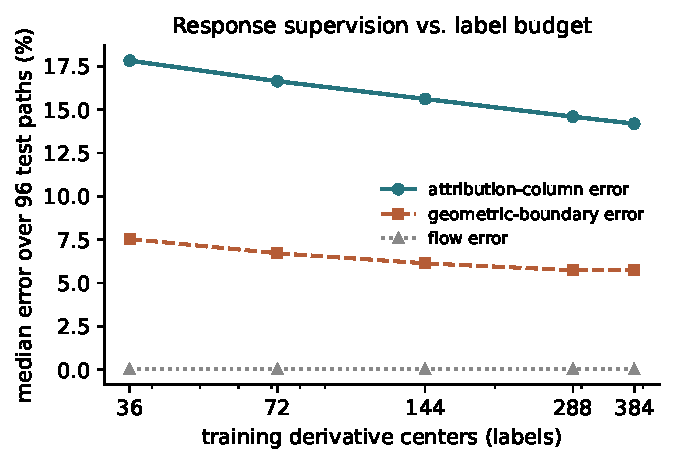
\includegraphics[width=0.72\linewidth]{../figures/fig_v109_labelbudget.pdf}
\caption{Response supervision under reduced label budgets on the 96
test paths, at the validation-selected weight: median attribution
column, geometric-boundary and flow errors against the number of
training derivative centers (36--384). The full-budget point (384
centers) is the main comparison of
Table~\ref{tab:fairmethods}.}\label{fig:v109labelbudget}
\end{figure}

\paragraph{Stability under a tripled training budget.}
Neither method sits at a validation plateau at the 1{,}200-update cap.
Repeating the frozen continuation protocol with the budget tripled to
3{,}600 updates (Figure~\ref{fig:v109convergence}; on Sioux Falls the
first twelve validation points --- the original 1{,}200-update budget
--- reproduce the archived runs to $10^{-12}$ in validation boundary
error) improves
both objectives on both networks, so the comparison above is not an
artifact of the cap. On the 96 test paths, flow-only training improves
its median column error from $21.18\%$ to $19.46\%$ and response
supervision from $14.19\%$ to $11.41\%$; on Anaheim's 48 paths, from
$1.64\%$ to $1.24\%$ and from $1.31\%$ to $0.88\%$. The ordering
persists and its relative margin widens on both networks (column-error
ratio $0.67\to0.59$ on Sioux Falls, $0.80\to0.71$ on Anaheim), with
flow accuracy again slightly better under response supervision.
Validation curves continue to decrease at 3{,}600 updates --- most
steeply for response supervision on Sioux Falls ($41\%$ further
boundary-error reduction from step 1{,}200) --- so the reported
operating points remain budget-limited, with the larger remaining
headroom on the response method.
\begin{figure}[t]
\centering
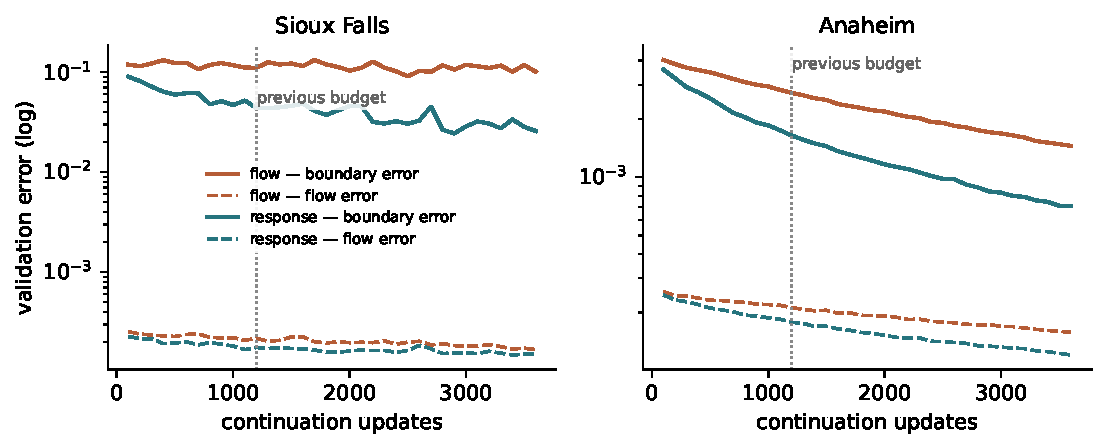
\includegraphics[width=\linewidth]{../figures/fig_v109_convergence.pdf}
\caption{Validation convergence under the tripled continuation budget
(seed-median validation boundary error, solid, and relative flow
error, dashed; log scale): Sioux Falls (left) and Anaheim (right),
flow-only (ochre) versus response supervision (teal). The dotted line
marks the previous 1{,}200-update budget; both objectives keep
improving beyond it, and the response curves stay below the
corresponding flow curves throughout.}\label{fig:v109convergence}
\end{figure}

\paragraph{Total error of the delivered summaries.}
The quantities of Table~\ref{tab:pathtable} concern the learned
profiles; the delivered artifact is the learned model's minimum-segment
summary. Table~\ref{tab:totalerror} evaluates the budget of
Eq.~\eqref{eq:totalbudget} on both networks under a common
per-query normalization (percent of the reference family scale
$\max_U|a^S_j(U)|$; the model term of Table~\ref{tab:pathtable}
reappears as $E_{\mathrm{model}}$ here). On Sioux Falls, flow
supervision leaves the model term dominant ($8.74\%$ versus a summary
term of $4.76\%$); response supervision lowers it to $5.75\%$, bringing
it to the level of the prescribed tolerance, so further reductions
require both a tighter tolerance and a better model. On Anaheim the
learned columns are closer to the reference and the budget is
compression-dominated ($E_{\mathrm{model}}$ $0.9\%$ versus a summary
term at the tolerance), so a tighter tolerance is the primary lever
there. On both networks the measured total error of the delivered
summary stays within the budget on every path. Relative to the
baselines, segmentation cuts the total error by a factor of
$3.0$--$3.8$ (single common value) and $1.7$--$2.0$ (equal-count) on
Sioux Falls, and by $10.5$--$10.6$ and $10.2$ on Anaheim --- where the
strongly ordered profiles make equal-count segmentation nearly as
coarse as a single value, so position-aware segmentation is what
carries the error control; the paired total error improves on $93.1\%$
of Sioux Falls path--query pairs under response supervision.
\begin{table}[t]\centering\footnotesize
\caption{Total error budget of the learned minimum-segment summaries,
cross-network summary at tolerance $5\%$ of the learned family
maximum. Sioux Falls: 96 test paths, direction-grouped families;
Anaheim: 48 test paths, ordered families. Entries are medians of
path-level values in percent of the reference family scale
($\max_U|a^S_j(U)|$), computed per path--query--seed and averaged
within path; Sioux Falls segments are summed over the family's
distinct direction chains (duplicate projection directions removed).
Single: one common value for the whole family; equal: equal-count
segmentation with the same per-direction
counts.}\label{tab:totalerror}
\setlength{\tabcolsep}{4.5pt}
\begin{tabular*}{\tblwidth}{@{\extracolsep{\fill}}llcccccc}
\toprule
Network & Method & $E_{\mathrm{model}}$ & $E_{\mathrm{summary}}$ & $E_{\mathrm{total}}$ & Single & Equal & Segments\\
\midrule
Sioux Falls & Flow & 8.74 & 4.76 & 11.35 & 34.3 & 19.7 & 117\\
Sioux Falls & Response & 5.75 & 4.75 & 8.68 & 33.0 & 17.2 & 117\\
\addlinespace
Anaheim & Flow & 0.94 & 4.33 & 4.57 & 48.0 & 46.6 & 9.9\\
Anaheim & Response & 0.78 & 4.32 & 4.55 & 48.0 & 46.6 & 9.9\\
\bottomrule\end{tabular*}\end{table}

\paragraph{Bound tightness.}
Computed with the same $41$-state trapezoidal quadrature for both
sides, the exact unrestricted errors $\mathcal K_j(e_j)$ lie below the
integrated bounds $B_j$ of Eq.~\eqref{eq:localboundarybound} (the
numerical verification and quadrature accuracy are reported in
Appendix~\ref{supp:accuracy}). The chain is tight: the median ratio
$\mathcal K_j(e_j)/B_j$ is $0.95$ for flow supervision (quartiles
$0.91$--$0.98$) and $0.95$ for response supervision (quartiles
$0.90$--$0.97$). The integrated bound is therefore a tight
\emph{a posteriori} upper bound on the realized worst boundary error
--- it uses reference-response information, as
Section~\ref{sec:totalbudget} notes --- and response supervision lowers
the geometric, unrestricted and bound levels in parallel. The
geometric family retains about half of the unrestricted error (median
ratio $E^{\mathrm{geo}}/\mathcal K_j(e_j)$ $0.51$ and $0.48$), so the
single-family errors reported throughout should be read as lower
bounds on the worst separating-region error. Sign reliability on the
separate frozen six-query baseline segment is boundary specific and is
retained in Appendix~\ref{supp:screenlinelearned}.
